\documentclass[aspectratio=169]{beamer}
\usepackage{fao}
\begin{document}

\begin{frame}
  \title{SOFIA-TAF\\[1ex]
    {\large\darkgreen Technical overview and demonstration}}
  \author{\vspace{-4ex}
    Arni Magnusson, Rishi Sharma, Nicole Tursich (FAO)}
  \date{SOFIA-TAF workshop, Bangkok\\[0.2ex]
    26 January 2023}
  \titlepage
\end{frame}

% ______________________________________________________________________________

\begin{frame}{Overview}
  \begin{itemize}
    \item[] {\bf\darkblue SOFIA-TAF}\\[0.1ex]
    \comment{open and reproducible, modular design, standardized
      structure}\\[2.5ex]
    \item[] {\bf\darkblue GitHub repositories}\\[0.1ex]
    \comment{\href{https://github.com/sofia-taf}{github.com/sofia-taf},
      analyses, package, data warehouse}\\[2.5ex]
    \item[] {\bf\darkblue TAF workflow}\\[0.1ex]
    \comment{data $\,\rightarrow\,$ model $\,\rightarrow\,$ output
      $\,\rightarrow\,$ report}\\[2.5ex]
    \item[] {\bf\darkblue R packages}\\[0.1ex]
    \comment{SOFIA, sraplus, TAF}\\[2.5ex]
    \item[] {\bf\darkblue SOFIA-TAF demos}\\[0.1ex]
    \comment{EffortShared, EffortByStock, IndexByStock, PriorsByStock}
  \end{itemize}
\end{frame}

% ______________________________________________________________________________

\begin{frame}
  \centering
  \vspace{1.5ex}
  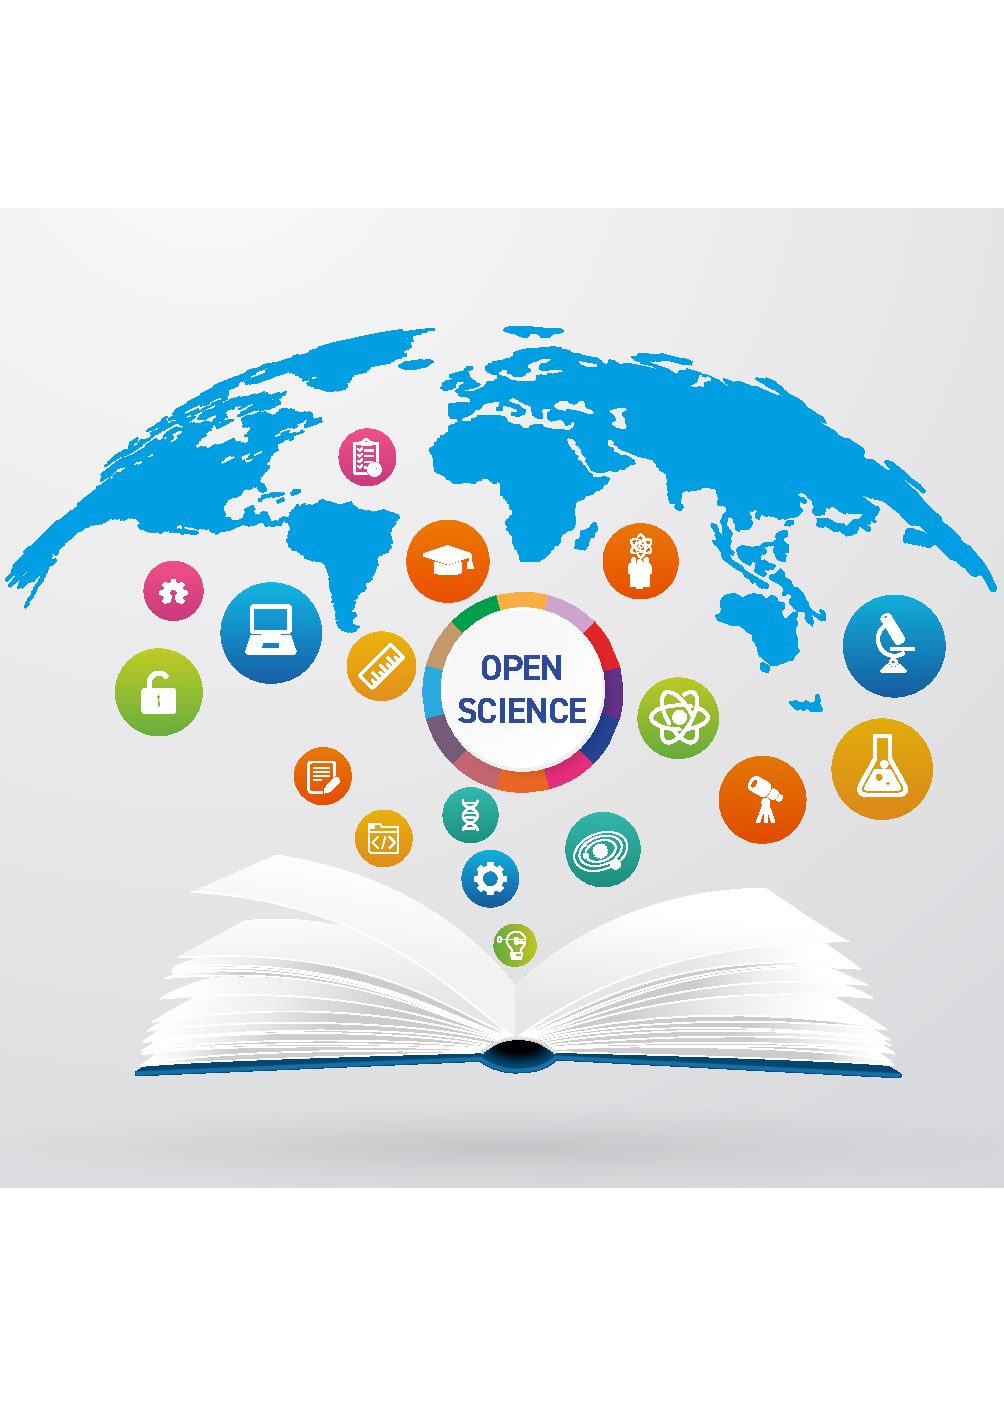
\includegraphics[height=0.9\textheight]{open_science}
\end{frame}

% ______________________________________________________________________________

\begin{frame}{SOFIA-TAF}
  \begin{tabular}{ll}
    {\bf\darkgreen 2020} & Initial discussions\\[2.5ex]
    {\bf\darkgreen 2021} & Prototype analysis of Area 37\\[0.5ex]
    ~    & Database\\[0.5ex]
    ~    & Design report\\[2.5ex]
    {\bf\darkgreen 2022} & SOFIA package 1.0\\[0.5ex]
    ~    & SOFIA-TAF launch at FAO-CAPAM meeting\\[0.5ex]
    ~    & Workshops in Areas 37, 31, 41\\[2.5ex]
    {\bf\darkgreen 2023} & Workshop in area 57\\[1.5ex]
  \end{tabular}
  \centering
  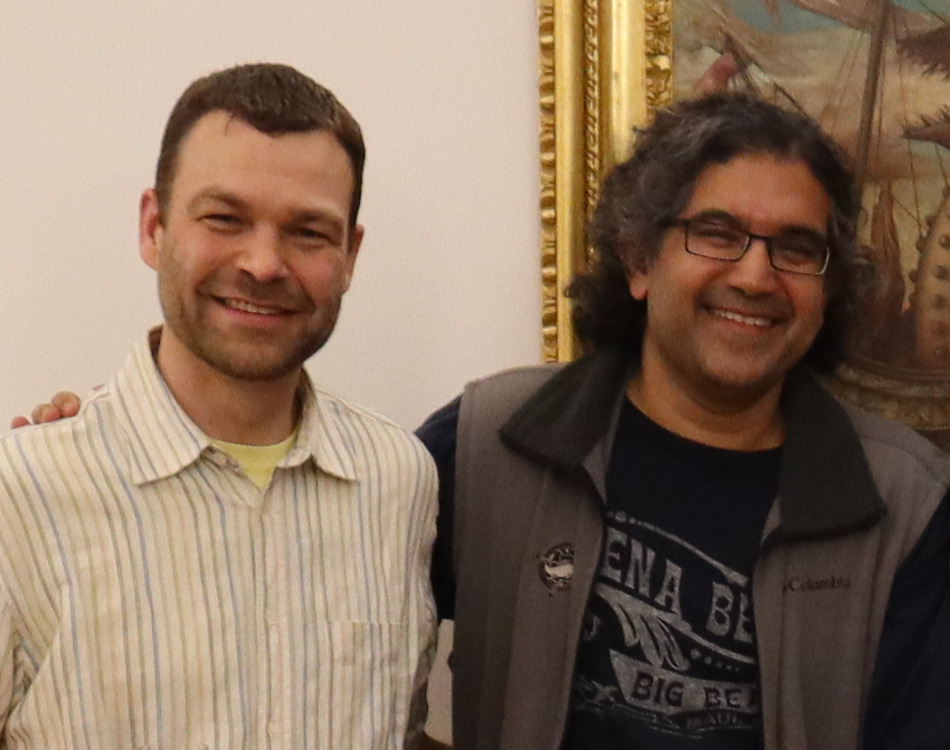
\includegraphics[width=0.35\textwidth]{arni_rishi}
\end{frame}

% ______________________________________________________________________________

\begin{frame}{SOFIA-TAF}
  \begin{itemize}
    \item[] Standardized structure to organize the SOFIA analyses\\[3ex]
    \item[] All the fisheries in the world\\[3ex]
    \item[] Converted from monolithic R Markdown to modular scripts\\[3ex]
    \item[] Tiers 1, 2, and 3\\[3ex]
    \item[] Ongoing development at
    {\blue\href{https://github.com/sofia-taf}{github.com/sofia-taf}}\\[3ex]
    \item[] R package SOFIA, one place to make changes, affecting all the
    analyses
  \end{itemize}
\end{frame}

% ______________________________________________________________________________

\begin{frame}{SOFIA-TAF}
  \centering
  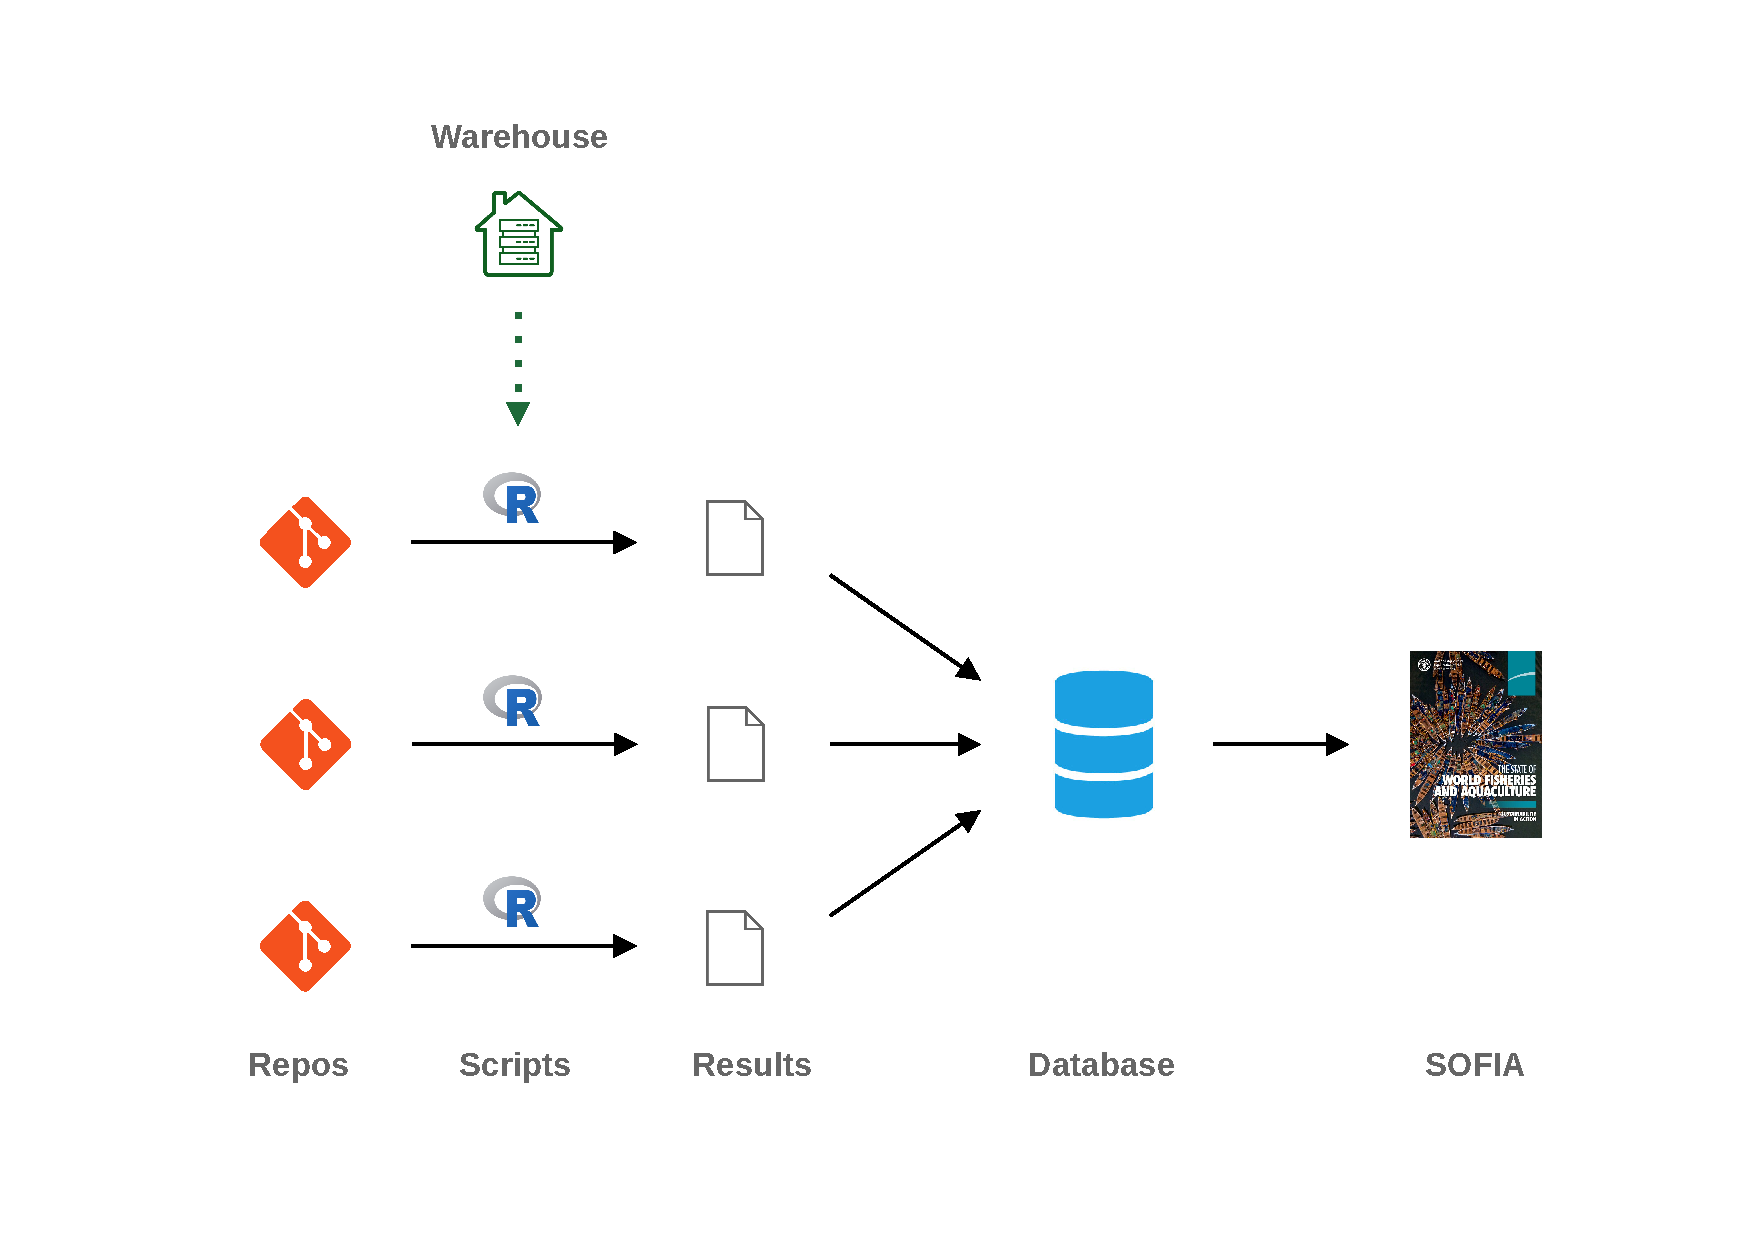
\includegraphics[height=0.75\textheight]{sofia_taf_diagram}
\end{frame}

% ______________________________________________________________________________

\begin{frame}{TAF}
  \centering
  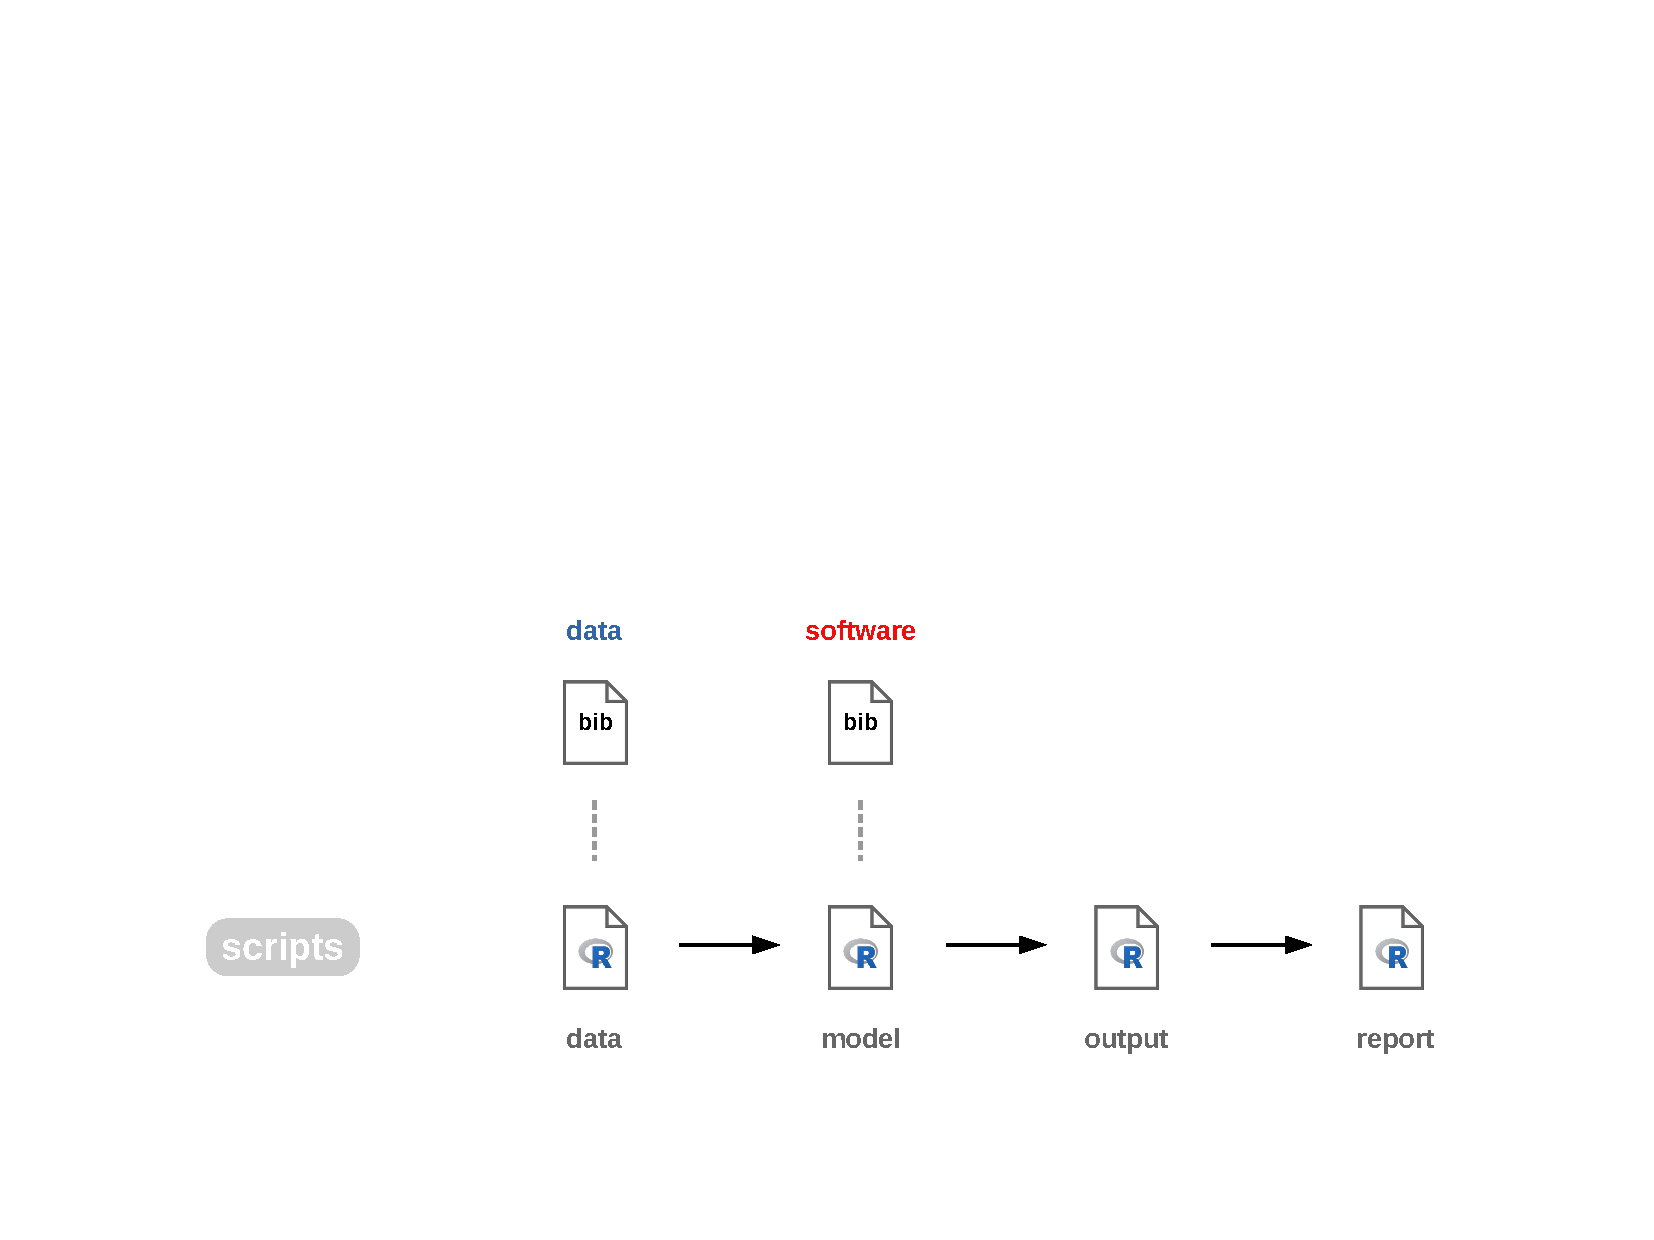
\includegraphics[width=0.6\textwidth]{taf_diagram}
\end{frame}

% ______________________________________________________________________________

\begin{frame}[plain]
  \begin{tikzpicture}[remember picture,overlay]
    \node[at=(current page.center)]
    {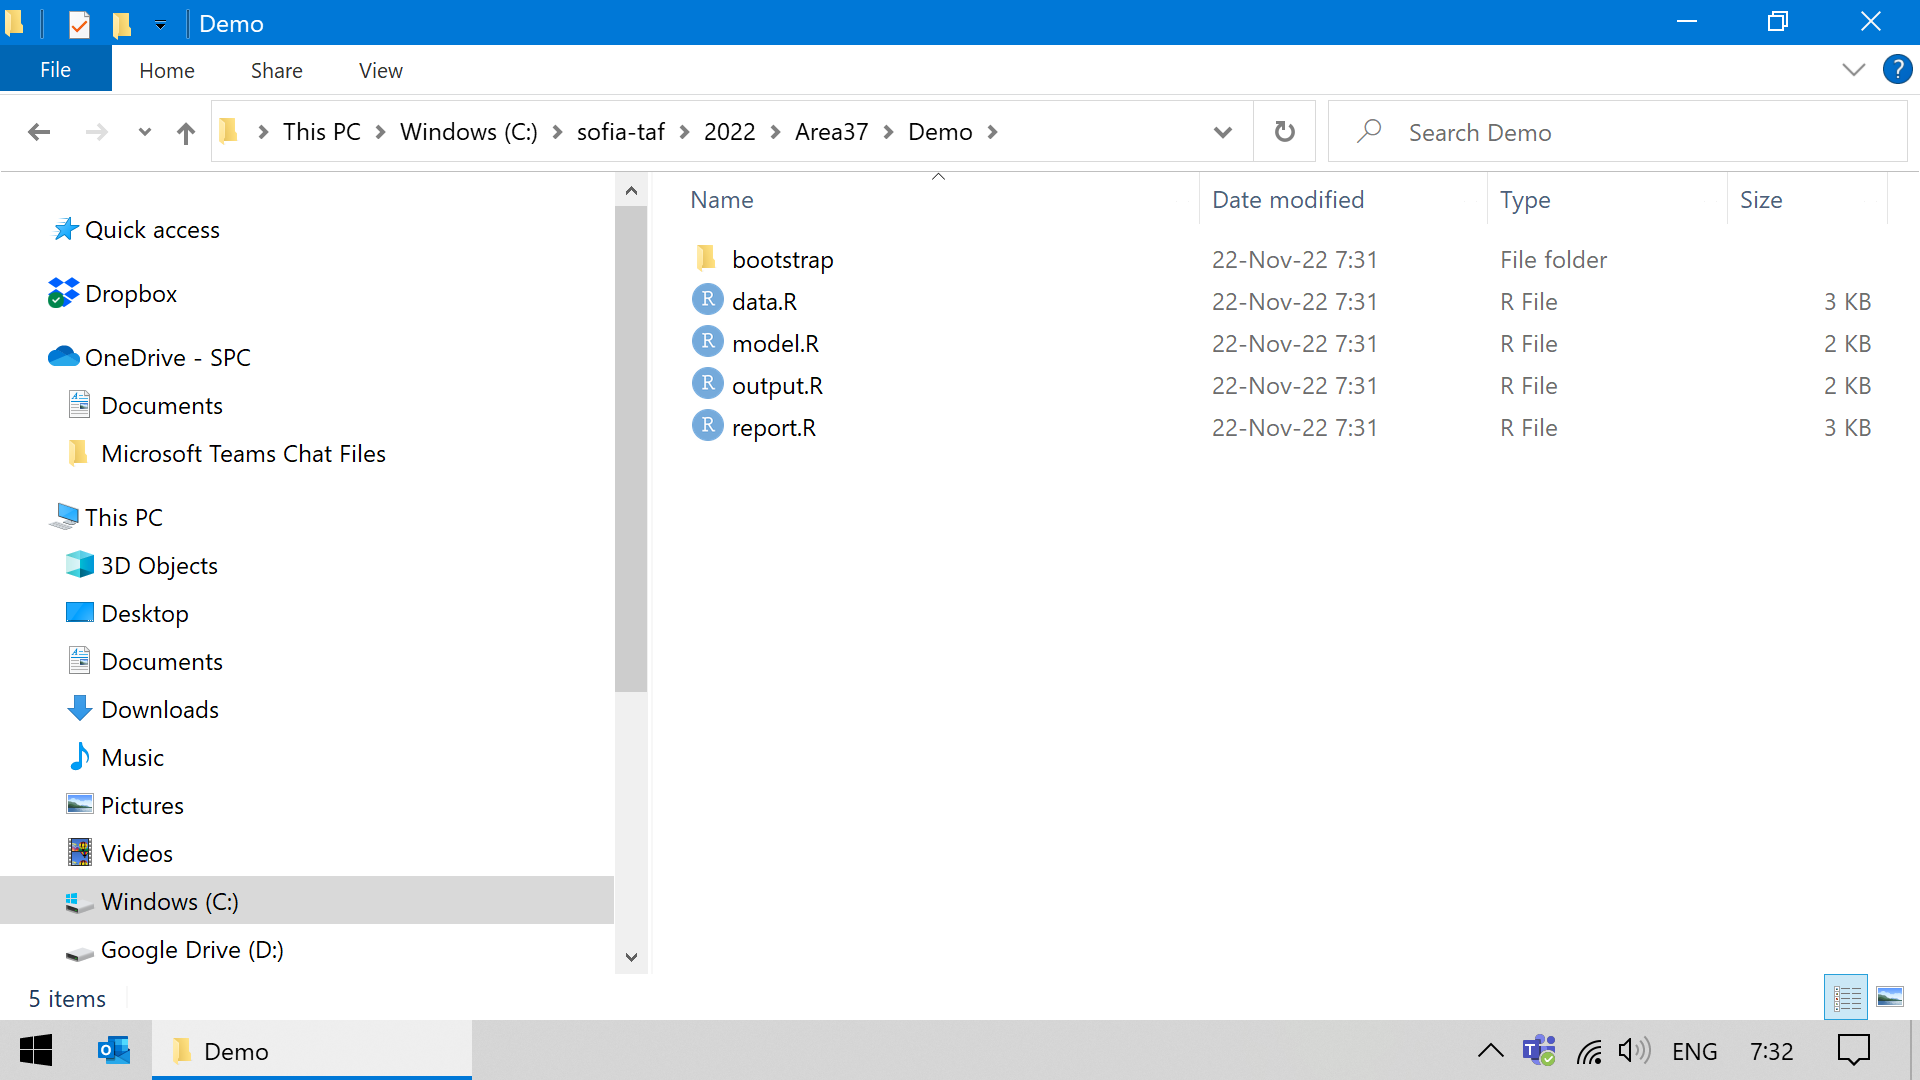
\includegraphics[width=\paperwidth]{file_explorer_1}};
  \end{tikzpicture}
\end{frame}

% ______________________________________________________________________________

\begin{frame}[plain]
  \begin{tikzpicture}[remember picture,overlay]
    \node[at=(current page.center)]
    {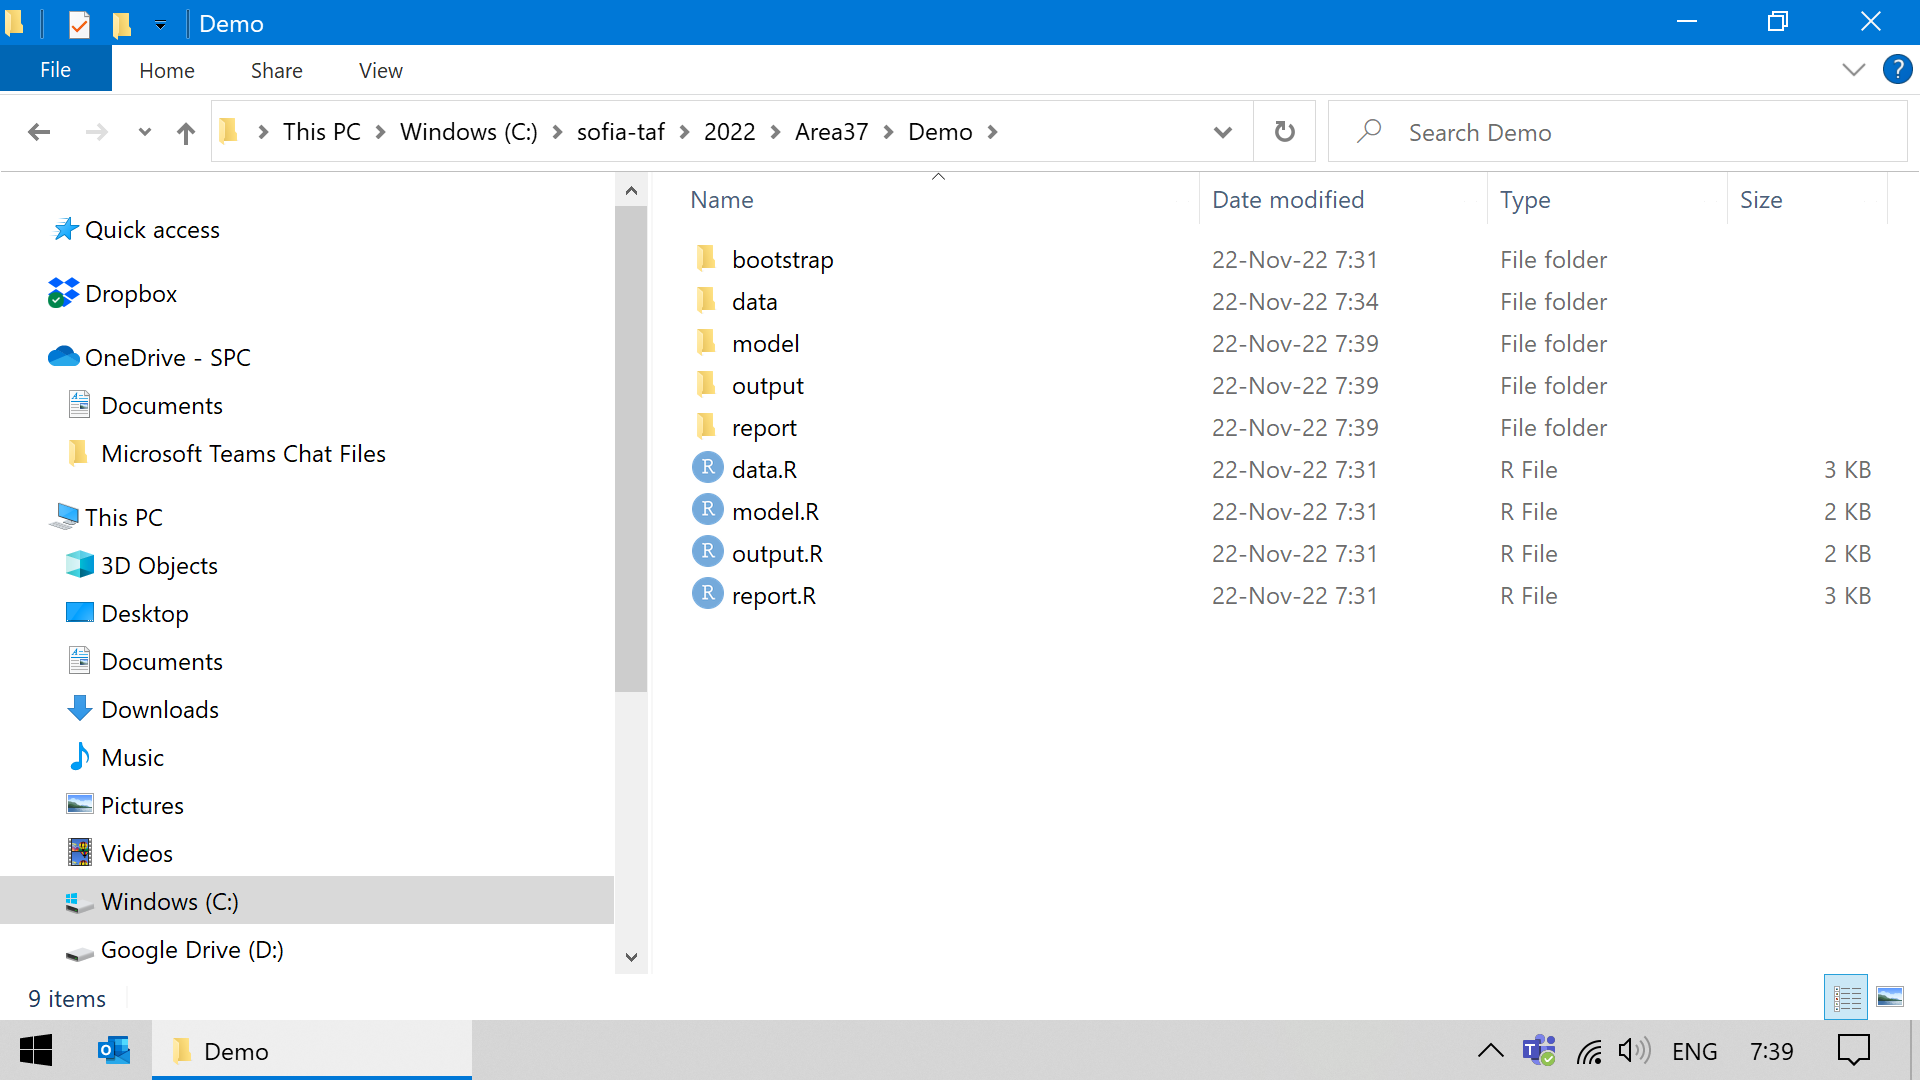
\includegraphics[width=\paperwidth]{file_explorer_2}};
  \end{tikzpicture}
\end{frame}

% ______________________________________________________________________________

\begin{frame}{SOFIA-TAF resources}
  \begin{itemize}
    \item[] {\bf\darkgray Documentation}\\[0.5ex]
    \qquad{\blue\href{https://github.com/sofia-taf/doc/blob/main/README.md}{overview}},
    {\blue\href{https://arni-magnusson.github.io/pdf/2021-sofia-taf.pdf}{design}},
    {\blue\href{https://github.com/sofia-taf/doc/blob/main/sofia_taf_tutorial.md}{tutorial}}\\[5ex]
    \item[] {\bf\darkgray Demos}\\[0.5ex]
    \qquad{\blue\href{https://github.com/sofia-taf/2022Area31EffortShared}{EffortShared}},
    {\blue\href{https://github.com/sofia-taf/2022Area31EffortByStock}{EffortByStock}},
    {\blue\href{https://github.com/sofia-taf/2022Area31IndexByStock}{IndexBystock}},
    {\blue\href{https://github.com/sofia-taf/2022Area41PriorsByStock}{PriorsBystock}},
    {\blue\href{https://github.com/sofia-taf/2023Area57Demo}{Area57}}\\[5ex]
    \item[] {\bf\darkgray Packages}\\[0.5ex]
    \qquad{\blue\href{https://github.com/sofia-taf/SOFIA}{SOFIA}},
    {\blue\href{https://github.com/DanOvando/sraplus}{sraplus}},
    {\blue\href{https://github.com/ices-tools-prod/TAF}{TAF}}
  \end{itemize}
\end{frame}

% ______________________________________________________________________________

\begin{frame}{Overview}
  \begin{itemize}
    \item[] {\bf\darkblue SOFIA-TAF}\\[0.1ex]
    \comment{open and reproducible, modular design, standardized
      structure}\\[2.5ex]
    \item[] {\bf\darkblue GitHub repositories}\\[0.1ex]
    \comment{\href{https://github.com/sofia-taf}{github.com/sofia-taf},
      analyses, package, data warehouse}\\[2.5ex]
    \item[] {\bf\darkblue TAF workflow}\\[0.1ex]
    \comment{data $\,\rightarrow\,$ model $\,\rightarrow\,$ output
      $\,\rightarrow\,$ report}\\[2.5ex]
    \item[] {\bf\darkblue R packages}\\[0.1ex]
    \comment{SOFIA, sraplus, TAF}\\[2.5ex]
    \item[] {\bf\darkblue SOFIA-TAF demos}\\[0.1ex]
    \comment{EffortShared, EffortByStock, IndexByStock, PriorsByStock}
  \end{itemize}
\end{frame}

\end{document}
